% Turabian Formatting for Theses and Dissertations, 2018/08/06
%
% Developed using the turabian-formatting package (2018/08/01), available through CTAN: http://www.ctan.org/pkg/turabian-formatting
%
% Additional document class formatting options:
%
% raggedright: ragged right formatting without hyphenations
% authordate: support for the author-date citation style
% endnotes: support for endnotes

% document class handles the big-picture formatting
\documentclass[draft]{turabian-thesis}

% For Turabian citations, use the biblatex-chicago package
\usepackage[noibid]{biblatex-chicago}
\addbibresource{backmatter/works-cited.bib}


% inputenc handles unicode (i.e. non-ASCII characters, such as letters with umlauts). This may need changing, depending on what you're using to compile (LuaTex, pdftex, etc.)
\usepackage[utf8]{inputenc}

% graphicx handles graphics. Requisite for hyperref, don't worry about this.
\usepackage{graphicx}

% For lorem ipsum text. use \lipsum[5] to create placeholder text. Increase the number in the brackets for more text.
% Very handy to get an overview of how it's going to look, but also can make you feel unreasonably confident- beware!
\usepackage{lipsum}

% it's unwise to mess with anything in this section- all of these are great packages, and if you don't use them, then LaTex doesn't include them, so there's no reason to turn them off.
% I have included some search tags in the hope that they're useful. Refer to the package's documentation for further information about how to implement them.
%%%%%%%%%%%%%%%%%%%%%%%%%%%%%%%%%%%%%%%%%%%%%%%%%%%%%%%%%%%%%%%%%%%%%%%%%%%%%%%%%%%%%%%%%%%%%%%%%%%%%%%%%%%%%%%%%%%%%%%%%%%%%%%%%%%%%%

% fancyhdr does fancy headers.
\usepackage{fancyhdr}

% for comments
\usepackage{comment}

% microtype handles microscopic improvements.
\usepackage{microtype}

% cmap makes pdfs searchable.
\usepackage{cmap}
% % % % search pdf, text, highlight text


% csquotes handles quotations
\usepackage{csquotes}
% % % % quotes, quoting, quotation

% ellipsis handles ellipses.
\usepackage{ellipsis}
% % % % ellpisis, ellipses, ..., . . . 

% allows half and half in tables. 
\usepackage{diagbox}
% % % % diagonal tables, split table

% allows multiple rows in tables.
\usepackage{multirow}

% For fancier tables.
\usepackage{booktabs}

% xcolor handles adding coloured text.
\usepackage{xcolor}
% % % % coloured text, color, red text

% for captioning
% \usepackage{caption} % hypcap is true by default so [hypcap=true] is optional in \usepackage[hypcap=true]{caption}

% for referencing the titles of sections
\usepackage{nameref}
% % % % reference titles

% for appendices
\usepackage{appendix}

% for including pdf pages
\usepackage[final]{pdfpages}

% for including quotes
\usepackage{epigraph}

% for in-line code
\usepackage{listings}
% % % % code font
\usepackage{hyperref}
% for todos
\usepackage{fixme}
\fxsetup{
    status=draft,
    author=Rhys,
    layout=pdfnote, % also try footnote, inline, or pdfnote
    theme=signature
}
\definecolor{fxnote}{rgb}{0.94, 0.97, 1.0}


% hyperlinks! The option [hidelinks] makes it still black i.e. not obviously a hyperlink. Remove [hidelinks] to make it the classic hyperlink style.

% \hypersetup{
%     colorlinks = false,
%     linkbordercolor = {white},
%     urlcolor = {blue}
% }

%%%%%%%%%%%%%%%%%%%%%%%%%%%%%%%%%%%%%%%%%%%%%%%%%%%%%%%%%%%%%%%%%%%%%%%%%%%%%%%%%%%%%%%%%%%%%%%%%%%%%%%%%%%%%%%%%%%%%%%%%%%%%%%%%%%%%%

% Information for title page
\title{Writing Wrong Right}
\subtitle{An Investigation in Composing with Extended Techniques}
\author{Rhys Gray}
% \course{Doctor of Philosophy (F4D)}
\institution{University of Tasmania}
\department{CALE --- Creative Arts, Conservatorium of Music}
\location{Hobart, Tasmania}
\date{\today}

% define new commands i.e. variables i.e. pieces of music
\newcommand{\violinPiece}{\emph{what are you doing with the humans}}
\newcommand{\violaPiece}{\emph{doppelganger}}
\newcommand{\bassPiece}{\emph{the veldt}}
\newcommand{\celloPiece}{\emph{liminal}}
% aliases for performers to maintain anonymity
\newcommand{\violaParticipant}{Angus}
\newcommand{\celloParticipant}{Sarah}
\newcommand{\bassParticipant}{Joe}
\newcommand{\work}{Joe}

\newcommand{\phdTitle}{Writing Wrong Right: An Investigation in Composing with Extended Techniques}

% for how deep the ToC should go
% -1 part     1 section     3 subsubsection  5 subparagraph
%  0 chapter  2 subsection  4 paragraph
\setcounter{tocdepth}{2}

% this is where the document starts. Comment out things that you don't need.
\begin{document}
\frontmatter{}
\maketitle
\tableofcontents{}
% \listofillustrations{}

\mainmatter{}
\subsection{Brief Background}
In 2019, I completed my Honours exegesis at the University of Tasmania, titled `Harmonic Based Extended Techniques and their Compositional Applications', a study of three extended techniques applicable to stringed instruments; half-harmonics, subharmonics, and multiphonics.
I am interested in pursuing this line of research further, as I believe that there is still more to be learnt about the techniques that I have already covered, and that many other extended techniques lack the literature that composers can use to make informed decisions about their use. 
The purpose of this study will therefore be to explore extended techniques further, filling literature gaps and incorporating the techniques into my own artistic language.

Cellist and new music specialist John Addison has expressed an interest in developing his technique of `double touch' harmonics with me, which he describes as `[\ldots] where one engages two of the harmonic nodes on the same string in the same series simultaneously, which allows upper harmonics in the series that have never been stable nor dependable to become reliable and certain.'
% This discovery expands exponentially not only the facility of producing the said harmonics but when applied to double-stops (the production of tones on two strings simultaneously) it increases the available options from around 40 to 243.


His technical and theoretical knowledge will be useful in testing and conducting practical research on the techniques, with eminent composer Sofia Gubaidulina stating 
    `I am convinced that we are dealing with a brilliant artistic personality here. 
    It is to be expected that John Addison’s activities as an interpreter will have a vital influence on the next generation of musicians.'\footnote{Personal correspondance between John Addison and Sofia Gubaidulina.}
As a spectralist composer, I am primarily concerned with extended techniques that make use of microtonalities, exploit the harmonic series, and spatial acoustics.
The recent shift of the Conservatorium of Music to the Hedberg provides an exciting opportunity to conduct research using the variable acoustic panels, and the ways that they can be used in site-specific works. 
The scope of my research would therefore be surrounding the treatment of these extended techniques; a holistic review of the techniques from the view of a composer and performers will shed light on the way that the techniques can best be produced.

As a composer, exploring subharmonics, multiphonics, double touch harmonics, and other extended techniques is particularly exciting, as they are fertile ground for new and unique sounds that can be used to develop my musical identity.
% I plan for the resultant thesis to be a practical document that composers and artists can use as a reference manual for the production and implementation of the techniques in their own practices.
My research into underexplored techniques will broaden the performative and compositional palette available to artists. 
Through the documentation of my process in researching this technique, it will be catalogued and brought into the literature, facilitating further development.


Through a comprehensive review of how composers construct their frontmatter, guidelines to how new and experimental techniques can be communicated to performers will be developed.
This will lower the friction of learning new works, and promote the uptake of contemporary works.
This will be further aided by the development of a \LaTeX{} style which can quickly scaffold the relevant extended techniques for consistent and universal verbiage.

The resultant thesis, `Writing Wrong Right: Composing With Extended Techniques', will consequently be a practical document, suitable as a reference for artists interested in implementing extended techniques into their practice.


\subsection{Key Questions}
\begin{itemize}
    \item How are extended techniques used in current literature, and are there ways to improve their delivery and make them more accessible to composers, performers, and audiences?
    \item Are there extenuating circumstances that keep these techniques from entering mainstream literature, or are they simply still in their infancy? 
    \item How have other artists used these techniques, and what can we learn from artists that have already incorporated them into their practice?
    \item How can I incorporate these extended techniques into my personal practice and develop a unique style with them?
    \item How well understood is the physical production, and are there ways we can improve production of the sound in a performance context?
    \item What variables impact the production of these techniques?
    \item What can we learn from the way that these techniques are physically produced? 
\end{itemize}


\subsection{Aims}
\begin{itemize}
   \item Develop my artistic voice and personal style through the incorporation of these extended techniques into my practice.
   \item Broaden the field of research by studying extended techniques that have not been extensively researched.
   \item Develop ways of communicating the best practices of techniques to increase their accessibility to others by formalising notation.
   % \item The best practice of how to produce the techniques will be synthesised by understanding the physical properties of the techniques and how they are produced. 
\end{itemize}


% My PhD is about building better music notation. 
% It can be thought of as taking an old house, and reconstructing blueprints of it, so that anyone can build extensions on it, and they know which walls they can knock down.
% I'm then building a catalogue of room designs that can replace parts of the existing structure, or be built as extensions;
% for composers that don't want to use rhythm as presented in Western staff notation, they can tear out those supporting beams, and replace it with 
% I'm looking at the Western staff notation that already exists, and breaking it down to its base elements, so I can construct building blocks for new notation out of that. 
% That, combined with my own set of rules that are developed from best-practice design and extrapolations from existing notation will help inform how to construct new techniques and notation. 
% The benefit of this is that it will help future-proof our notation for future technologies, 
% \section{Literature Review}
This PhD continues upon the previous research that I conducted during my Honours, and there is significant overlap with the two topics.
Therefore, the first item that is worthy of mention would be `Harmonic Based Extended Techniques and their Compositional Applications', which includes a ground-level review of the seminal literature in the field.\autocite{grayHarmonicBasedExtended2019}
However, due to the limited scope of the exegesis, there were significant omissions, so for the sake of completeness its contents will be reviewed under the lens of `composing with extended techniques'.
Additionally, there are a number of sources that were either missed or cut from the initial literature review for sake of brevity.
% There appears to be a great deal of activity in similar spheres of research in Basel, Switzerland, and there are several manuscripts and texts that appear only in German.

Unlike standard pedagogical models, wherein the student learns from the teacher, the methods used in this exegesis are a more collaborative, and less rigid practice.
Composers typically will have a performer in mind when they compose a work, and collaborate with them, working to find what works for the artists and instrument.
However, in subsequent performances, that direct connection to the composer is often unavailable, and the performer is left to interpret the paratext, without direct instruction from the composer.
Paratextual instruction can vary in degrees of specificity, and will often be printed in the frontmatter of the work.
Where there is a well established understanding of the technique (such as the Bartok pizzicato technique, which has been accepted into the canon of `standard' techniques, and is no longer considered extended), this is not an issue, but can pose issues in the case of techniques where there is a great deal of variance possible, such as multiphonics and subharmonics.
In some cases, the performer must rely on previous works to build a contextual language in which to interpret esoteric markings, or use previous recordings of interviews and performances to ascertain the composer's intent.
Understanding the composer's intent is a crucial part in the preparation process, and the ability to accurately reproduce the composer's intent may negatively impact a work's longevity in the literature.
Many academics have recognised the deficit in training in extended techniques, both in their base form and their composer-specific implementation (which may vary from composer to composer, or piece to piece). 
Violist Sarah Wei-Yan Kwok discusses this in her thesis `Breaking the sound barriers: extended techniques and new timbres for the developing violist', where she commissions six etudes for viola exploring extended techniques, along with an investigation into pedagogy.\autocite{kwokBreakingSoundBarriers2018}

The composer-performer collaboration dynamic has been explored at length; the most famous example being the virtuoso pianist Paul Wittgenstein, whose career came to a halt during World War 1, when he lost his right arm.
Afterwards, he began commissioning leading composers to write for him, resulting in Richard Strauss', `Parergon zur `, `Sinfonia Domestica for Piano and Orchestra', Maurice Ravel's `Piano Concerto for the Left Hand in D major', and further works written by Hindemith, Korngold, Britten, and Prokofiev, to name a few.\autocite[107]{predotaPaulWittgensteinVoice2014}
Collaboration with the intended performer is crucial to a composer's ideas being realised accurately, as articulated by Jack Barnes, who stated:
\begin{quotation}
    My collaboration with Mathieson-Sandars allowed for subtle but important improvements to \emph{Lines, Contexts and Freedoms}. 
    Certain aspects such as the composer hearing his piece for the first time, experimenting with different pianistic timbres and creating more comfortable hand distributions were among the most useful outcomes of our collaboration. 
    As the performer, it was useful for my interpretation to learn [the composer's] intent behind the gestures; that the effect of dynamic shaping was not desirable for all of them.\autocite[20]{jackbarnesExaminationComposerPerformerCollaborations2017}
\end{quotation}
Discussion being needed with the composer to learn the composer's intent suggests that there was information being provided to Barnes that was not present in the paratext.
Future performers of the work that was commissioned by Barnes may not have the same level of access to the composer, hence the need for a thorough and precise documentation of the intended sound being available.

Sheet music is an abstracted conception of a musical work; the printed paper is merely a set of instructions that are interpreted by the performer, in order to express a musical idea that only the composer truly knows.
Without a perfect abstraction of what the composer imagines, a `perfect' reproduction is impossible.
Indeed, even if there \emph{was} a perfect reproduction, the variance in instrumental timbre and other facets of the process render it a fool's errand.
The Platonic ideal is unattainable, and perhaps why little effort has been made to make further progress towards the liminal.\autocite{citation needed, obviously}

Attempts at combining notation with composer intent have been made, with Eftiha Victoria Arkoudis' `Contemporary Music Notation for the Flute: A Unified Guide to Notational Symbols for Composers and Performers' building on the work of Robert Dick.\autocite{arkoudisContemporaryMusicNotation2019}

Instructive manuals are typically in one of two categories; performer-oriented, in which the techniques presented are articulated in a performer-focused context, and composer-oriented; orchestration manuals which dictate the end results.
For brevity, these usually do not intersect, or at least are not written comprehensively with both the composer and performer in mind. 
The lack of literature that encompasses the entirety of the production of sound process, from the action to the resultant, is slowly being rectified, particularly with online resources such as Heather Roche's work in clarinet multiphonics, and Fallowfield's with CelloMap gaining popularity.\autocite{rocheHeatherRoche, fallowfieldCelloMap}
\subsubsection{Notation Manuals}
Notation has long been the domain of Kurt Stone and Gardner Read being the authoritative voices, writing extensively on the subject beginning in the 1970s.\autocite{stoneMusicNotationTwentieth1980,readCompendiumModernInstrumental1993,readContemporaryInstrumentalTechniques1976,readMusicNotationManual1979a}
Additional texts by David Cope and Erhard Karkoschka supported these with their own contributions.\autocite{copeNewMusicNotation1976,karkoschkaNotationNewMusic1972}
Editor of Faber Music, Elaine Gould's seminal `Behind Bars' gave an authorative voice to the methods of notating along with the building blocks for techniques which she felt had not been developed to the point of consensus.\autocite[iii]{gouldBars2011}

\subsection{Physics}
In order to be able to accurately prescribe instructions on how to produce these techniques, there must be an understanding of the underlying physics.
Helmholtz provides our basic undestanding of the stick---slip motion which makes a bow produce sound on a string.\autocite{helmholtzSensationsTonePhysiological1954}
Knut Guettler and Håkon Thelin have provided extensive research into how the string can produce multiphonics.\autocite{thelinAnalysisBowedStringMultiphonics,thelinMultiphonicsDoubleBass2011,guettlerBowedstringMultiphonicsAnalyzed2012,guettlerGuideAdvancedModern1992,guettlerWaveAnalysisString1994}
\fxnote{This needs to be expanded}{R. T. Schumacher, Kenneth Marskall, and Anders Askenfelt contribute additional aspects to the literature.}\autocite{schumacherTransientBehaviourModels1995,askenfeltMeasurementBowingParameters1989,marshallModalAnalysisViolin1985}
For subharmonics, the violinist that discovered the technique, Mari Kimura, has contributed practical examples on how to produce them.\autocite{kimuraHowProduceSubharmonics1999}
\fxnote{Empirical data on what? Expand!}{However, for research into the technique's production, Robert Mores, Guettler, Erwin Schoonderwalt, Carleen Hutchins, and John Cantrell provide empirical data.}\autocite{moresFurtherEmpiricalData2019,guettlerBowedStringDevelopment2002,schoonderwaldtViolinistSoundPalette2009,hutchinsSubharmonicsPlateTap1960,cantrellSubharmonicGenerationChaos2015}

\subsection{Extended Techniques}
To understand extended techniques, we must first establish a basis of what is considered a `regular' technique, or rather, what the qualifying factors are for a technique to be considered extended.
To do this, we will look at what techniques are commonplace in the literature, and which are less so.
Techniques that require descriptions in the frontmatter or otherwise `extend' the instrument beyond the normal canon would reasonably be understood to be considered extended techniques.
Read discusses this, stating:
\begin{quotation}
    Many so-called ‘new’ instrumental devices have developed from well established techniques; they are extensions of, or refinements of, procedures long considered part of a composer’s repertorium of expressive devices. 
    The newness, then, is not one of kind but of degree, a further and more extensive development of basic effects found in scores from the late nineteenth century to the present day.\autocite[3]{readContemporaryInstrumentalTechniques1976}
\end{quotation}
Unpacking the language that we use, extended techniques are just that; an extension of the traditional techniques that are already established in the canon. 

\fxnote{This probably needs retooling to fit better in the literature review.}There are three aspects that are relevant to the literature review; literature surrounding the techniques themselves, literature with how the techniques are presented, and scores. 
Scores are necessary to understand how composers implement extended techniques in practice.
By reviewing their frontmatter and the symbol notation, we gain an understanding of how composers present information to performers, and can build a system of notation that maps consistently with the rest of the established canon.
Consequently, seminal scores will be included in the literature review so that we may understand how they work. 
These scores' notation systems for extended techniques will be broken down into their elements, and through comparative analysis of how different composers implement the same techniques, we will be able to find how textual, symbolic, and graphic notation systems can be used to achieve the desired results.

Dimpker postulates the following criteria for extended technique notation; \begin{quote}
    `(1.) As exact as possible and (2.) As simple as possible while the system may (3.) Not be contradictory to
traditional notation, but should instead extend and be closely related to it.'\autocite[3]{dimpkerExtendedNotationDepiction2012}
\end{quote}
This meshes well with the philosophy of Elaine Gould's `Behind Bars', which advocates for a consistent style language, despite the two texts occasionally coming at odds with one another in the exact treatment of some cases.\autocite[120--121, 61]{dimpkerExtendedNotationDepiction2012,gouldBars2011}
Dimpker posits that four methods of notation are acceptable in order to realise exact and precise notation; `action notation, symbolic notation, diagrammatic notation, and schematic notation'.\autocite[33]{dimpkerExtendedNotationDepiction2012}

Textual notation, i.e.\ instructions printed in the score, are the most straight forward, but limited to what can be summarised in few words.
Symbolic notation assigns the technique to a symbol, typically with the instructions placed in the frontmatter.
Graphical notation systems are often used when the binary of symbolic notation is restrictive, and requires a greater fidelity than textual notation can provide. 
An example of this can be seen in Kaija Saariaho's notation of overpressure, wherein she uses a black bar to represent the amount of overpressure required, temporally relational to the position in the score.\autocite{TODO:saariaho citation}

\subsubsection{Double Touch Harmonics}
The technique of `double touch harmonics' as described by John Addison appears to be almost totally novel; it may be a matter of the technique being developed under a different name, but the only reference that seems to be relevant is a 1980 thesis, which has not been made available online.\autocite{woodrichMultinodalPerformanceTechnique1980}
Addison has completed several fingering charts and made preliminary instructive documentation on the technique, which has been provided to the researched.
Due to the lack of literature, collaboration with performers will be essential in order to build the technique to a stable, usable state.

\subsubsection{Multiphonics}
Multiphonics have been well-documented in reed instruments, with Robert Dick's seminal `The Other Flute', setting the gold standard in extended technique documentation, painstakingly notating the outputs, fingerings, and qualities of flute multiphonics and other extended techniques.\autocite{dickOtherFlute1989}
There are several Barenreiter technique manuals for other aerophones that cover multiphonics, including bassoon, saxophone, violin, and oboe, with the publisher appearing to try and compile a manual for every instrument.\autocite{weissTechniquesSaxophonePlaying2010,galloisTechniquesBassoonPlaying2009,ardittyTechniquesViolinPlaying2013, TODO:OboeBook}
\fxnote{Double check to see if this is true}The book on violin by violinist Irvine Arditty notably lacks any information on multiphonics, perhaps due to the difficulty of production on the small instrument.\autocite{ardittyTechniquesViolinPlaying2013}

\paragraph{String instruments}
The development of literature dealing with multiphonics on stringed instruments is more recent, with a special January 2020 Tempo journal issue, dedicated entirely to string multiphonics.
It was collated by Dr.\ Ellen Fallowfield, who notably contributed the landmark thesis CelloMap (and eponymous website) in 2009.\autocite{fallowfieldCelloMapHandbook2009, fallowfieldCelloMap}
Her article, `Cello Multiphonics: Technical And Musical Parameters' expands upon the work that she began in her thesis, `CelloMap'.\autocite{fallowfieldCelloMultiphonicsTechnical2020}


\paragraph{Plucked chordophones}
Rita Torres has explored multiphonics on the guitar extensively, with several papers dedicated to their research, including her thesis, `A New Chemistry Of Sound: The Technique Of Multiphonics As A Compositional Element For Guitar And Amplified Guitar'.\autocite{torresMultiphonicsCompositionalElement2012}
Paulo Ferreira-Lopez and Torres provide a robust exploration of previous systems of notation of multiphonics, suggesting notational methods similar to those that Fallowfield suggests.\autocite{ferreira-lopesGuitarMultiphonicsNotations}
Catalogues of multiphonics in the guitar literature show that there has been little interest in the technique, with the first score dating back to 1832, but only around twenty or so pieces composed since the techniques inception.\autocite[80--82]{torresSoundWorldGuitar2018}
It has been suggested that the widespread adoption of the technique has been marred by the mode of playing naturally having a decay, making multiphonics more difficult to hear for an audience, as well as the guitar having a poor dynamic range.\autocite[21--22]{Torres2014TowardsOT}
This has been all but confirmed with the analysis of multiphonic signal decay at distances equivalent to that of an audience revealing that without amplification, the multiphonics will be inaudible.\autocite[279]{torresGuitarMultiphonicsInfluence2014}
Thomas Ciszak and Seth Josel expand upon the research carried out by Torres, collating a catalogue of performable multiphonics from strings 3 --- 1, and examining multiphonics on the electric guitar.\autocite{ciszakNeonLightMultiphonic2020}

\paragraph{Piano}
The piano, an unlikely candidate for multiphonics, has had some success in making inroads in the technique through the use of preparing the piano.
With the development of more robust literature, the prospect of developing a new sound-palette for the piano is alluring.
Interest begins in 2016 with Juhani Vessikala's MA thesis on the topic.\autocite{vesikkalaMultiphonicsGrandPiano2016}
Sanae Yoshida acknowledges Vessikala's work in an article in the multiphonics issue of Tempo, where Yoshida expands upon the practical ways in which a composer can use microtonality (and multiphonics) on a piano.\autocite{yoshidaMicrotonalPianoTunedIn2020}
Following is Caspar Walter's algorithm to calculate the frequency components of pure multiphonics.\autocite{casparjohanneswalterVariantsContinuedFraction2019}



\subsection{Methodology}
% Autoethnography, document analysis, interviews, research
Through interviews with players at varying stages of proficiency and familiarity with the techniques, I will be able to uncover the barriers to producing these techniques. 
Document analysis of existing resources and compositions will help direct and support the line of enquiry. 
Autoethnography of my creative process will document the research process and clarify my intent.  

To understand extended techniques, we must first establish a basis of what is considered a `regular' technique, or rather, what the qualifying factors are for a technique to be considered extended.
To do this, we will look at what techniques are commonplace in the literature, and which are less so.
Techniques that require descriptions in the frontmatter would reasonably be understood to be considered extended techniques.

The aim of this research project is not to make the techniques popular enough to make clarification of technique unnecessary, or for it to enter the canon of techniques so that it is no longer considered to be `extended' (as the Bartok pizzicato has).
Rather, this is intended to act as a resource for composers and artists to be drawn upon as a reference for when they wish to use the technique.
A considered and informed judgement call over a technique can only be made when the technique is understood well.
The composer will communicate the information necessary to realise the technique to the player, typically through the frontmatter. 
In order to better understand what information composers deem useful to communicate to players, a review of scores with similar techniques will take place.
By breaking the score's frontmatter content up into its actions, we can understand how composers communicate their desired techniques to players.

% \section{Timeline}
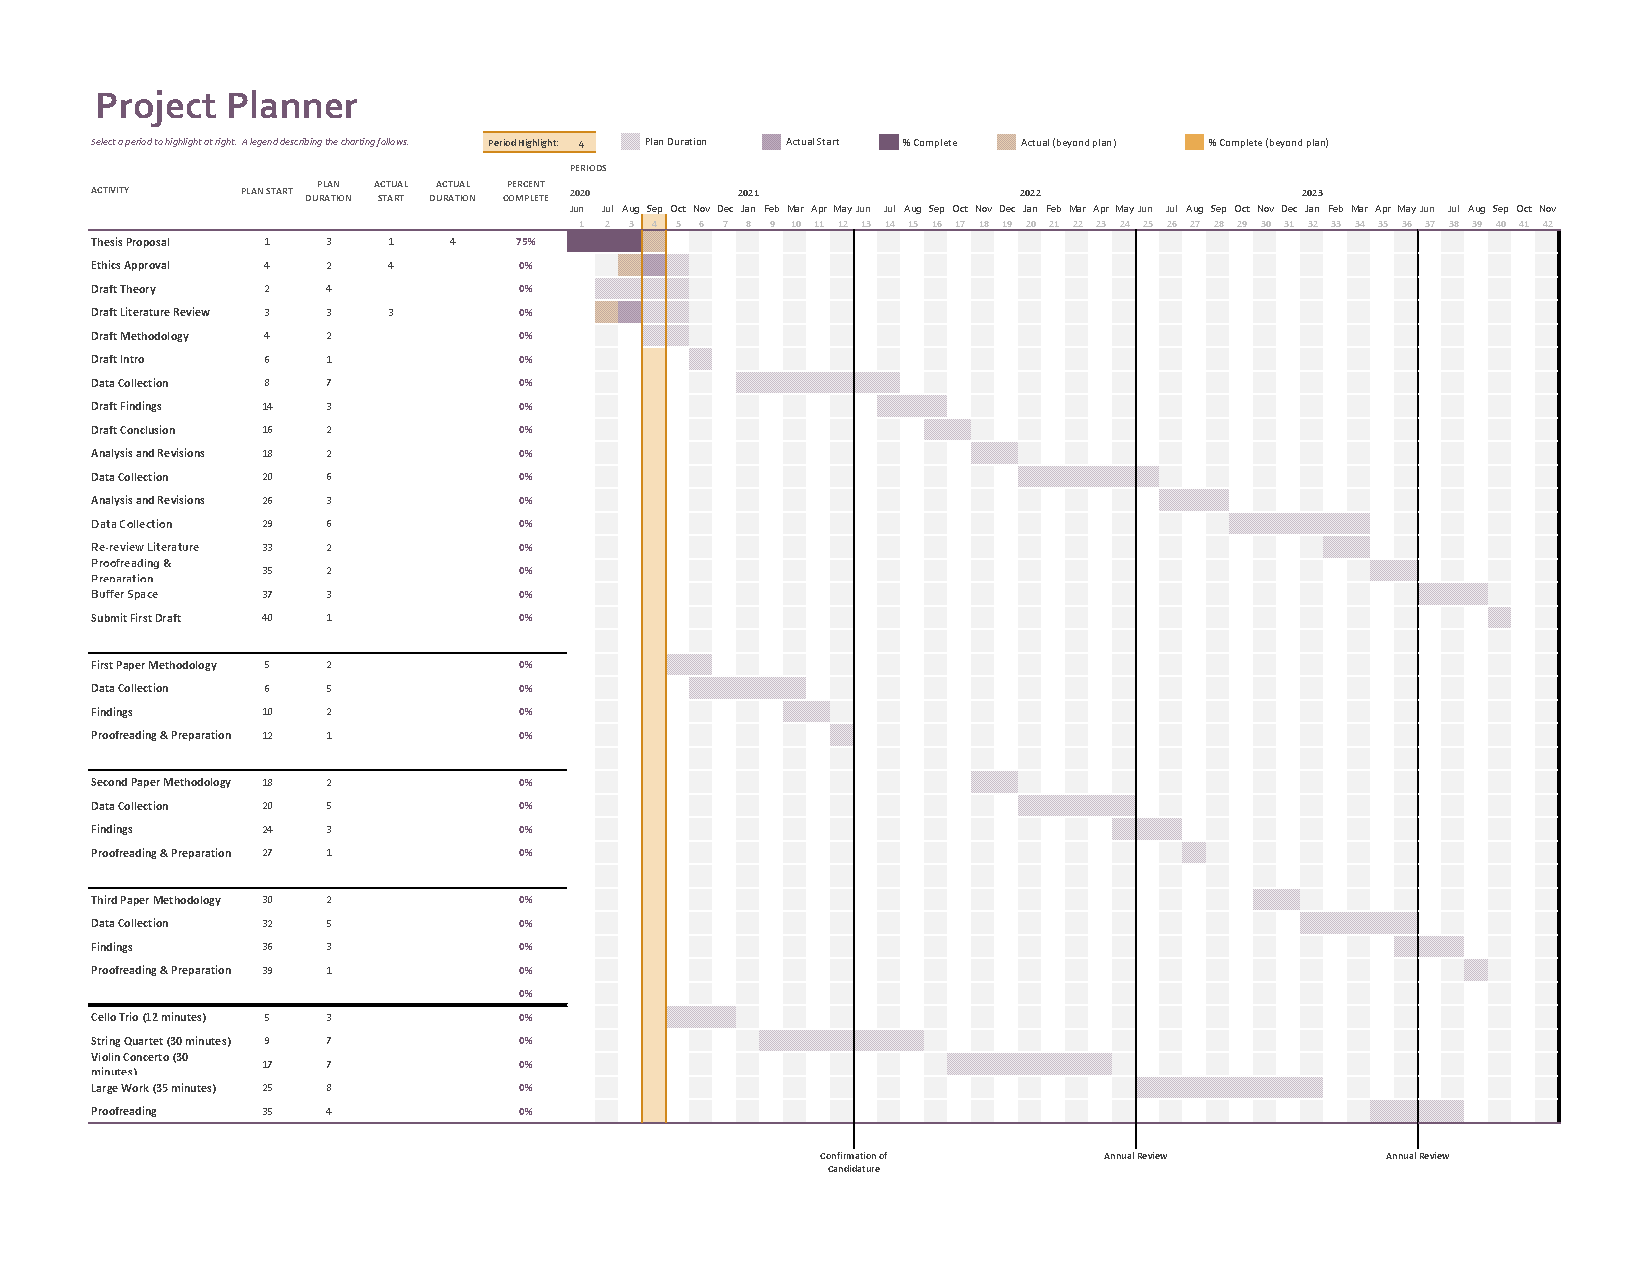
\includepdf[pages=-,pagecommand={}]{../resources/gantt.pdf}
\subsection{Outcomes Of This Project, and Why It Is Relevant}
This project will provide me with a better understanding of the mechanics and musical capabilities of the extended techniques. As these techniques currently have a deficit of literature, both instructive and artistic; there are few resources for people to learn from, and even fewer practical examples of how to implement the techniques in a musical context.
My research will address this, filling the research gaps where identified.
The outcome of my research into the technique of `double touch harmonics', as developed by John Addison, is particularly relevant as it presents an exciting possibility for a new method of producing familiar harmonics.
This will increase the number of available fingering positions of harmonics within existing compositions, as well as providing more colour options for performers to choose from.

\subsection{Outputs}
My research into underexplored techniques will broaden the performative and compositional palette available to artists. 
Through the documentation of my process in researching this technique, it will be catalogued and brought into the literature, facilitating further development.


Through a comprehensive review of how composers construct their frontmatter, guidelines to how new and experimental techniques can be communicated to performers will be developed.
This will lower the friction of learning new works, and promote the uptake of contemporary works.
This will be further aided by the development of a \LaTeX style which can quickly scaffold the relevant extended techniques for consistent and universal verbiage.

The resultant thesis, `Writing Wrong Right: Composing With Extended Techniques', will consequently be a practical document, suitable as a reference for artists interested in implementing extended techniques into their practice.
\section{Introduction}
% \addcontentsline{toc}{chapter}{Introduction}


% Set page numbering to arabic the first time we commence a chapter.
% This is required to get the page numbering correct.
\pagenumbering{arabic}
\doublespace{}

In my first year of composition, I wrote an ambitious work called `Music for String Instrument and Audience', in which the audience received a full score of the work along with the programme for the recital.
The work was notated as a colour-coded flowchart, and it `talked the audience through' the work; elements of chance were included for both the performer and audience to act upon.
These included instructions such as `play until you get bored, then move to the next box', `play until you hear a rustling of paper in the audience', and `if you are wearing plain socks, play this instead'.
My intent was to both demonstrate an understanding of the hegemonic hierarchy of the composer-performer-audience relationship, and challenge it, as usage of extended techniques was missing from my high school portfolio.
The performance was marred by the lights not going on, resulting in the audience not being able to read the scores in the dimly lit room, but despite the catastrophic premiere, the work provoked an interest in me regarding the systems that were at play, and I attribute it at least partially with my fascination with extended techniques.

In my thesis, `Writing Wrong Right: Composing With Extended Techniques', I examine the ways in which we can remove the barriers that composers and performers face with extended techniques.
As part of the thesis, I explore the semiology of notation, and deconstruct it to establish a `cookbook' of elements, which can be used to construct new notation for techniques that adheres to the unwritten `style guide' of existing Western musical notation.
This paper is a practical example of this; in it, I use autoethnography to show my experiences constructing both a technique, and a type of notation. 
This is intended to be representative, as a technique maps an action to a symbol, while a form of notation maps a mode of interacting with an instrument to the score;
it is intended that the reader can extrapolate from my findings along with the cookbook to construct notation to suit their purposes as required.
% chapter1.tex (Chapter 1 of the thesis)

\renewcommand*{\thefootnote}{\arabic{footnote}}
\setcounter{footnote}{0}
\section{Goals}

In this section, I examine the interfaces used to communicate music, and synthesise a working model of ways to notate techniques that can interface with traditional Western musical notation, and extend it.
The argument being put forth\fxnote{put forth by whom?} is that much like a language, music notation evolves naturally, with new `words' being developed when no suitable existing `word' is found.
The system which I propose is not a constructed language like Lojban or Esperanto, which take an opinionated and prescriptive approach to language. 
Rather, the method is more like compiling a list of morphemes\fxnote{What is a morpheme?} encountered in existing works, breaking down our existing musical language into its elements so that compoundment, affixation, and other methods of constructing new `words' may occur naturally.
With this system, we will be able to establish a dictionary of existing symbols, as well as their function.
Composers that seek to notate in new and different manners will be able to take the symbols and interfaces a la carte, and construct their own, specific to their needs.
In instances of entirely novel concepts, this morphemic catalogue can be applied using mimetic principles to communicate intent clearly.

\section{Literature Review}

\subsection{Overview of Semiotics}

A brief overview of semiotics is necessary in order to contextualise the intent and methodology that is used.
Semiotics, the study of signs (read: meaningful communication), was invented concurrently by Ferdinand de Saussure and Charles Sanders Peirce independent of one another.\fxnote[]{saussure}
The most appreciable difference between their models was that while Saussure held that signs were made up of a signifier (the form of the sign) and signified (its meaning), Pierce's model also had an interpretant; the object that the audience interprets the signified as (since it is impossible to replicate meaning perfectly).\fxnote[]{pierce}
Signifiers are then broken up into three discrete categories; 
\begin{itemize}
\item \emph{\gls{icon}}: which have a direct physical connection to the signified. Photographs are an example of icons.
\item \emph{\gls{index}}: which show evidence of the signified. The most common example being smoke indexing fire.
\item \emph{\gls{symbol}}: which have no resemblance between the signifier and the signified; their meaning must be culturally learned. Arabic numerals, the radioactive symbol, and flags are all symbols.
\end{itemize}

Finally, our signs have two channels of information.
\begin{itemize}
\item \emph{\gls{denotation}}: the basic or literal meaning of the sign (i.e.\ a picture of a rose signifies the flower of the genus \emph{Rosa} of the family \emph{Rosaceae})
\item \emph{\gls{connotation}}: the secondary, culturally inferred meaning; a rose might also signify passion or love, depending on the context.
\end{itemize}

Interpreting these signs is described as semiosis, which Philip Tagg states is `simply the process by which meaning is produced and understood.'\autocite[156]{taggMusicMeaningsModern2013}
Semiosis happens constantly; the process of converting these words into the understanding of the concept of semiosis is, in itself, semiosis. 
Pierce argues that in between the audience and the signifier, during the process of semiosis there is the interpretant, an object that the audience creates that represents the signified (because a dog cannot exist inside our heads, but merely the idea of a dog; the reality of the dog will never be fully realised inside the mind because it lacks the gestalt of the physical thing; 
it's a construct, unable to approach the truth of the dog by virtue of its limitations).\fxnote[]{pierce}
Semiosis is an important step, as the interpretant which Peirce describes is unique to the audience; we construct meaning completely independently, informed by our past experiences and knowledge.\fxnote{citation needed Pierce}
Thus, the same picture of an aunt's dog may be interpreted by the aunt as being a loving pet, whereas a neighbour might interpret the image more negatively, as `the annoying dog that wakes me up at 6am'.

Looking at Western notation, we have several instances where a symbol may hold a different context depending on the interpreter's experience-- 
the same notation is used for a harmonic and a note that is meant to be played open on a French horn.\autocite[]{schuilingNotationCulturesEthnomusicology2019}
If a musician was given a piece of sheet music without any indicator of the instrument that it was written for, their experience (or lack thereof) with one of the instruments may influence how they choose to interpret the symbol.
John Fiske categorises \begin{quotation}
    denotation [as] what is photographed, connotation [as] how it is photographed
\end{quotation}.\autocite[91]{fiskeIntroductionCommunicationStudies2011}
What the composer chooses to put on the page could be argued to be denotative, while what is omitted and how the material is presented is connotative.

Semiotics is particularly applicable in web design, where intuitive `notation' is sought after to reduce the `friction', or difficulty a user has navigating a site.
We can learn many things from the research that has been done into how to use skeuomorphic\fxnote{What is this?} design to convey an element's function.
Our goal with constructing intuitive music notation is to reduce the `friction' just like a web designer, using design patterns that are intuitive even to people that are unfamiliar with the content.
We can use the connotations of existing symbols to help infer how we can construct new symbols.
As an example, the line that makes up a glissandi can be either straight, or wavy, as seen in \autoref{fig:Glissando}.
\begin{figure}
    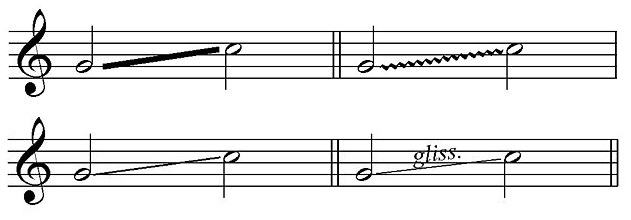
\includegraphics[]{./resources/glissando.jpg}
\caption{Various styles of glissandi}\label{fig:Glissando}
\end{figure}
The similarity of the last two examples on the right to the notation for \emph{portamento} results in a connotation with those two types being continuous, rather than having discrete pitches.
Additionally, the interpretant's instrument may also influence the meaning to them- timpanists and trombonists are more likely to interpret glissandi as continuous changes, while pianists interpret step-wise due to the nature of their instruments.\fxnote{need to find a citation for this}
In this way, we understand that the meaning of a symbol is tied inextricably with the culture of the interpretant; attempting to make use of this cookbook for an audience not `primed' to understand it (i.e.\ one unfamiliar with Western art music conventions) is doomed to failure.
In order to produce a document that can be used reliably, the work must either be totally objective (a fool's errand in the pursuit of extracting cultural understanding of signs), or cognisant of the pitfalls and assumptions made.
To this end, the `cookbook' necessitates disclaimers specifying the assumptions made; terminology or notation used specifically in avant-garde or Renaissance music will not have any transitive qualities aiding its uptake to an audience that is not familiar with the source material.

Some symbols are not compatible with one another; a properly engraved work will never have an upbow and downbow on the same note, as the two symbols fulfill the same function (unless, of course, the two symbols are joined together, which denotes a rapid rebowing).
This is what is known as a paradigmatic relationship; by virtue of the presence of one, it excludes the possibility of the other.
Looking at web design, we can draw a somewhat rough parallel to drop-down menus; there's only one slot that can be filled.
Other examples of paradigms would be the degree at which a French horn opens or mutes their instrument, which is not a binary, but a scale of `openness'.

Understanding the properties of a sign that are inherited from its history, context, and role informs what information is necessary to communicate to the reader in order for them to be able to make use of the `cookbook'.
Without a cohesive and holistic (or rather, as holistic as is possible) treatment of the signs, the intent of the `cookbook' falls short; composers must be armed with the knowledge of the context in which the sign developed, and its use in order to be able to make informed decisions.



\subsection{Argument}
% The perhaps hyperbolically described `cult of the written score' in the 20th century New Complexicist movement saw the rise of composers prescribing more and more parameters.
I aim to catalogue actions from a composer's perspective, providing a suite of tools with which a composer can construct a notation to suit any imagined circumstance; be it using an animated score that changes with time, a score seen within a VR headset, or any other interface that may develop in the future.\fxnote{Rephrase}
In the 20th century, the `cult of the written score' developed, in which the composer prescribed more and more parameters to be interpreted literally.\fxnote{citation very much needed}
This was in part fueled by contemporary composers being strongly opinionated in how their works should be interpreted, and partly because of the styles-- the sheer breadth of the number of parameters specified in New Complexicist works makes the interpreter pre-biased to assume that there is little room for interpretation.\fxnote{Need a couple of examples here}
This has permeated through to an underlying culture of assuming that when performing a work by a living composer that, if they wished for it to be interpreted a specific way, they would have specified that.\fxnote[]{can't really cite this}
There have been several notable theses on the philosophy and reasons behind the New Complexicist movement, and it would be ill-advised to retread tired arguments.
All that is relevant to this study is that music notation is an imperfect representation of the perfect, Platonic ideal, which exists only in the mind of the composer. 
This is to say that notation is the physical manifestation of an interpretant which exists only in the composer's mind, imperfectly represented in the physical form.

Floris Schuiling describes music notations as \begin{quotation}
`interfaces for imagining virtual musical relations'
\end{quotation}
which is an apt description; similar meaning can be derived from verbal instructions, and the notation used is merely a vehicle through which to deliver the instructions on how to play the work.
The end result of this is that the precise vehicle through which performers obtain their instructions can be modified, mutated, and otherwise changed to better represent the imagined musical relations as the composer envisages.
This is done often when the traditional structure of Western music notation fails to account for some niche that it was not designed for; the aleatoric works of John Cage, stochastic aleatoricism of Lutoslawski, and many others who sought to extend the artform to its metaphorical breaking point.
Their modifications and adaptations of notation have, to varying degrees, taken root, and become accepted into the canon as valid notation; it is unlikely that the reader would have any doubt of the intended effect if presented with a Bartok pizzicato symbol above a string instrument's note.
However, these notations have been developed independent of one another, and in the current musical sphere, we are faced with an ever-increasing list of symbols to memorise, along with lengthy descriptions littering the frontmatter.
Every composer that creates new notation (be it the notation of a technique, a method of notation, or an entire interface) is effectively treading new ground.
On occasion, multiple notations are created for the same technique, such as the multitude of ways that composers communicate \fxnote{TODO find example technique with duplication}.
However, duplication of technique is not necessarily a bad thing; `hairpin' crescendos and textual instructions both serve largely the same function.
In other cases, such as the notation for \fxnote{TODO find a better example than subharmonics} subharmonics, notations differ in specificity. 
Crumb's notation method has the least specificity, denoting simply a `scratchy tone' \fxnote{TODO find Crumb's quote}, while Kaija Saariaho specifies the relative degree of pressure to apply.
Mari Kimura's method specifies the resultant pitch, but omits the relative pressure required to obtain the tone.
These methods of notation are all for the same technique, but focus on different aspects, according to what is desired by the composer.
It is this philosophy that this thesis intends to address; 
providing a toolbox of components that a composer can use to construct new notation, as well as cataloguing existing notations so that composers may better communicate their intent, to make the interface that they create closer resemble the interpretant that exists in their head.

Of particular interest is the work of Ellen Fallowfield, whose thesis, `CelloMap' website and recently, application, form a comprehensive and holistic review of the ways in which a performer may `map' actions onto a cello.\autocite[]{fallowfieldCelloMapHandbook2009,fallowfieldCelloMap}
This non-opinionated and genericized method of cataloguing actions sees its contents applicable where a more specific approach would fall short, ensuring that it does not fall out of date.
% In a similar way, I aim to catalogue actions from a composer's perspective, providing a suite of tools with which a composer can construct a notation to suit any imagined circumstance; be it using an animated score that changes with time, a score seen within a VR headset, or any other interface that may develop in the future.

There has been much research done into the ways that computers can interpret sheet music, an extension of OCR technology which has resulted in several market-ready tools such as PhotoScore. 
More pursuant to this study are the developments of machine-readable formats such as the GUIDO music notation system, if only as examples of the parameters that must be accounted for.
The thesis `denm' makes a comprehensive study of many of the strategies and reasons that performers will mark up a score with annotations. 
Additionally, it goes into discussion of the various accessibility and printing issues associated with using CYMK colour in printed scores.\autocite[22--29]{beanDenmDynamicEnvironmental}
denm (Dynamic Environmental Notation of Music) is a 

Kurt Stone identifies many of the issues present in modern notation in his 1963 article in \emph{Perspectives of New Music}, and he states that \begin{quotation}
    `no other aspect of contemporary notation is more desperately in need of fundamental revision than that of rhythm.'
\end{quotation}, arguing that the existing systems of notating rhythmic ideas are either insufficient, poorly tooled, difficult to implement, or otherwise not suitable for purpose.\autocite[20--22]{stoneProblemsMethodsNotation1963}
Stone explores proportional notation as used in Stockhausen's \emph{Zeitmasse} and Cage's \emph{Music of Changes} (1951), identifying an issue where accidentals can interfere with precise placement of notes. 
This proportional notation system is very similar to the piano roll, or \emph{pianola} that is found in many Digital Audio Workstation workflows, such as Ableton, FL Studios, and Pro Tools.
The piano roll notation is arguably a superior method, as it is as literal as can be, assigning pitch to the y axis (with the label of the y axis being the matching piano key), and time to the x axis, often representing the metrical grid with lines.
However, while this workflow is suitable for DAWs, it is cumbersome to use in performance settings, and cannot be considered a genuine alternative for mapping music to an interface for performance purposes.
Stone notes this, recognising how proportional notation is ill-fitted to performer parts due to rhythmic explicitation via a `middleman' of a commonly agreed metrical unit being replaced with the much more subjective relational measurement; a crotchet is explicitly a crotchet, but a 3.3cm distance may be approximated to an imprecise element.
This can be mitigated with a common `cue' stave in parts, but as size of the ensemble grows, practicality decreases.

Stone describes notation as \begin{quotation}
    [\dots] a system of directional signs which [is] used to enable a performer conversant with them and and with the musical conventions of the era during which they were in use, to recreate a composer's \emph{artistic} vision on the basis of what the \emph{mechanical} directions implied.
\end{quotation}

He continues, stating that \begin{quotation}
    [some] of today's music is constructed in such a way that the slightest modification of \emph{any} of its measurable elements is likely to distort the inner logic of the entire work.
    In such music, only rigid sign realization is admissable; this music does not permit ``interpretation''. 
    At the same time, however, music of this nature is generally so complex that truly accurate sign realization is rarely if ever achieved in performance.
    Thus, the score and the performer have actually exchanged roles: whereas the score used to be the map designed to guide the performer towards the composer's artistic vision, it now is often completely explicit.
    On the other hand, performances are now often mere stabs in the direction of the composer's envisioned perfection of execution.
    The imprecision and variability of human performance are actually quite detrimental to the requirements of totally organized and predetermined works.\autocite[30--31]{stoneProblemsMethodsNotation1963}
\end{quotation}

This broad criticism of the failings of New Complexicists touches at the core of the issue; an imperfect relational system will produce imperfect results.

In the paper `Animated Notation, Score Distribution and AR-VR Environments for Spectral Mimetic Transfer in Music Composition', which deals with applying graphic scores to a new, Virtual Reality context, Jonathan Bell and Benedict Carey note that \begin{quotation}
    `the closer a musical unit gets to representing a direct action (that is, the movement of an object in space) the more mimetic it becomes.'\autocite[]{bellANIMATEDNOTATIONSCORE2019}
\end{quotation} This observation is paralleled with the 

While the generation of new methods of presenting music past the simple paper score is not a focus of this study, there is still much to be learned from the research that has been carried out in these fields.
Animated scores, as pioneered by Cat Hope and others are a relatively straightforward development of the static score as it exists in printed form, augmented with features such as playback lines, and dynamic elements.
`Inventing Malleable Scores: From Paper to Screen Based Scores', a paper by Arthur Clay introduces the concept of malleability to score creation and interpretation.

This thesis aims to provide the composer with more tools to aid in the specificity of the work, so that they may more accurately and concisely communicate the desired techniques.
\section{Methodology}

Cataloguing the entirety of the Western classical music canon of music notation is a monumental task, but can be broken into smaller, more manageable tasks by working from first principles.
If we limit our scope to interfaces that require interaction from humans to create the work, we immediately cut out swathes of computer-centric design patterns.
We can then further 

Through interviews with players at varying stages of proficiency and familiarity with the techniques, I will be able to uncover the barriers to producing these techniques. 
Document analysis of existing resources and compositions will help direct and support the line of enquiry. 
Autoethnography of my creative process will document the research process and clarify my intent.  

The aim of this research project is not to make the techniques popular enough to make clarification of technique unnecessary, or for it to enter the canon of techniques so that it is no longer considered to be `extended' (as the Bartok pizzicato has).
Rather, this is intended to act as a resource for composers and artists to be drawn upon as a reference for when they wish to use the technique.
A considered and informed judgement call over a technique can only be made when the technique is understood well.
The composer will communicate the information necessary to realise the technique to the player, typically through the frontmatter. 
In order to better understand what information composers deem useful to communicate to players, a review of scores with similar techniques will take place.
By breaking the score's frontmatter content up into its actions, we can understand how composers communicate their desired techniques to players.
\section{Case Study}

The composer and recorder player Claire Farrell approached me, asking for my opinion on how to notate an extended technique that she had been developing. 
The technique involves the recorder player covering the window hole with their index finger or hand, which results in the recorder producing a whistle like effect. 
Air pressure determines the pitch, and the degree to which the window hole is covered determines the fundamental's presence or lack thereof, with full occlusion of the window producing solely the harmonic. 

This is an ideal place in which to explore the ways in which we map actions into notation; the question becomes one of how this can be achieved in the most recognisable and orderly manner. 
Our goal of establishing a defined notation system is to ensure that it is as clear and easy to understand as possible. 

Thus began an informative exploration through the various ways that we can map sound onto an instrument. 
This is an especially interesting topic to me, as I am interested in the ways in which the semiotics of notation influence its parsing. 
We can treat this development of the notation of a new technique as a case study for best practices, and establish some ground rules on how the written form of Western art music can be adapted to accomodate new techniques that fall outside of the initial set.



% \begin{itemize}
% \item Textually, through the use of just text instructions. 
% Examples would include `mute'.
% \item Textually and pictographically, with text describing complex operations, aided by the shorthand of symbols. 
% Examples would include `mute unmute'.
% 	\item Pictographically; this would encompass all techniques that are divorced from the reality of the object, such as harmonics. 
% As this is a very broad category, it can be broken down further:
% 		\item Pictographically with symbols, such as our harmonic example.
% 		\item Pictographically, with mappings to physical objects, such as the pedal sign representing the lifting of the pedal, or the half-hole representing a partially occluded hole.
% \end{itemize}

\subsection{Building from Pre-existing Notation}

Maintaining compatibility with existing Western music notation is only possible if we follow the rules that are set out in existing symbols and structures.
This means that we cannot mutate existing symbols, or ascribe a different meaning to their common one; there are to be no uses of the piano pedal symbol to indicate a patch change on an electric keyboard.
Similarly, we cannot expect the user to intuitively understand symbols that don't follow the existing design language.

We first establish that if using a pictographic notation, that there is a point at which the instrument's window cannot be occluded any further. 
This would, logically, follow the pre-established convention of filled in black representing `more'. 
Further more, we know that there is a point at which there is no occlusion; the exact opposite. 
However, the precise point of this point is variable.

Pictographic notation is most useful when there are elements that cannot be conveyed succinctly with text; while it is true that you could notate it as `cover window with hand to produce high pitched seagull sound', it would be cumbersome to read and interpret quickly. 
Reducing that to `cover window' might result in unfortunate misinterpretations. 
Those examples also treat the act of covering the window as a binary; Claire described how the sound can change when you cover it partially, fully, or even stick your finger inside the window, blocking the free passage of air slightly to create a wholly new sound. 
So, we can safely establish that it is not feasible to use a textual direction with some degree of certainty; 
minute differences between covering the window from 30 percent to 50 percent and back to 20 percent would be unnecessarily verbose, or filled with numbers that were divorced from contextual information.

An aural equivalent can be drawn from double bass repertoire, in which a high harmonic on the bridge glissandos rapidly down to a lower partial, producing a `seagull' like effect. 
These are notated as regular harmonics, sometimes with `seagull effect' above the line. 
The double bass seagull effect is largely timbral though, and its efficacy of communicating the desired effect lies not in the notation, but in the unary nature of the intended resultant sound; a rapid dropping of a high pitch to a lower one. 
It is tied to a real world parallel, and is thus easily mapped onto the instrument.

Action parallels include the stopping of a horn with a hand, and covering windpipes on clarinets and flutes; see \autoref{fig:Asset10}. 
These are closer to the intended action, and indeed the recorder lowers a tone on full occlusion of the airway much like the horn. 
However, Claire noted an issue with the typical notation; the open circle, half-closed circle, and fully black circle had no relationship to the instrument. 
The half-occlusion of the circle was confusing as the window is a square, and fingering holes are round.
Claire was attempting to map a horn technique onto a recorder, with predictably confusing results. 

\begin{figure}
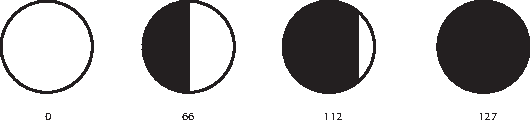
\includegraphics[width=\linewidth]{./resources/Asset 10.pdf}
\caption{Half-closed circle style}\label{fig:Asset10}
\end{figure}


I modified the notation to a rectangle, to represent the rectangular window, and added black to it to represent occlusion, moving from left to right as with the half-closed circle notation; see \autoref{fig:Asset3}.
For the sake of convenience, the level of occlusion has been mapped to a MIDI rate, of 0 being totally un-occluded, with 127 being fully occluded.

\begin{figure}
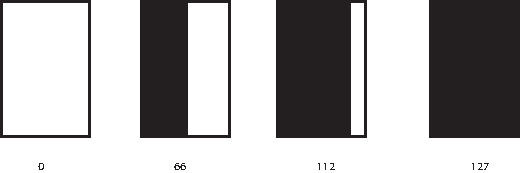
\includegraphics[width=\linewidth]{./resources/Asset 3.pdf}
\caption{Modified to a rectangle}\label{fig:Asset3}
\end{figure}

However, this was obviously inappropriate, as the action of occluding the window is not a left-to-right action.
I changed it so the black increased upwards as the notation dictated further occlusion of the window as seen in \autoref{fig:Asset1}. 
This mapped similar to how a MIDI expression level is displayed as a bar graph in DAWs. 
\begin{figure}
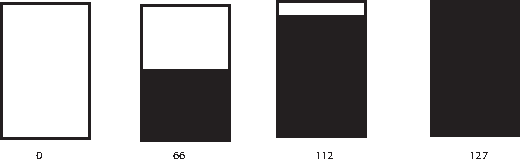
\includegraphics[width=\linewidth]{./resources/Asset 1.pdf}
\caption{MIDI style range}\label{fig:Asset1}
\end{figure}

But this too posed difficulties, as the instrument's window wasn't on the bottom of the instrument, and the hand comes \emph{down} to occlude the window. 
Rotating the image 180 degrees, I found the clearest notation yet; a picture that mapped both the intended one dimensional attribute of occlusion, as well as the action onto the instrument.

\begin{figure}
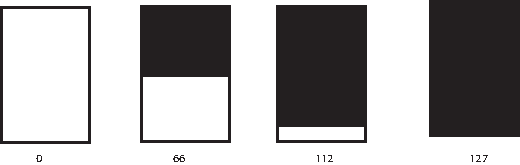
\includegraphics[width=\linewidth]{./resources/Asset 2.pdf}
\caption{Inverted MIDI style range}\label{fig:Asset2}
\end{figure}

And yet, we found there was still an outlying use-case that was not accounted for; the action of pushing the finger (or, indeed, abstracted out to any object) into the window. 
This posed an interesting issue, as it challenged our one-dimensional range attribute with needing to either accommodate the inclusion of a further attribute, or a method of delineating the cutoff point for total occlusion and where the `further in' position began. 
Further compounding the issue is the fact that there is no self-evident physical point at which further insertion is impossible; 
while the occlusion has a constant point where no further occlusion is possible (i.e.\ the window is a finite opening that can be eclipsed totally), one could theoretically put objects into the window as far as physically possible.
Further attempts were made, experimenting with a perspective representation of the window to communicate a `further in' style in the single symbol; 

\begin{figure}
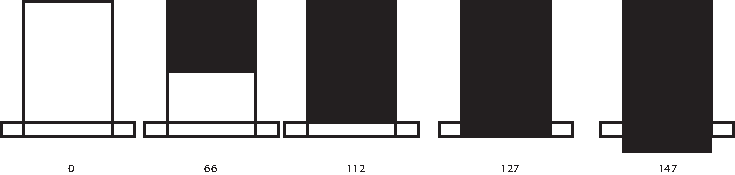
\includegraphics[width=\linewidth]{./resources/Asset 4.pdf}
\caption{First attempt; without upper limit}\label{fig:Asset4}
\end{figure}

\begin{figure}
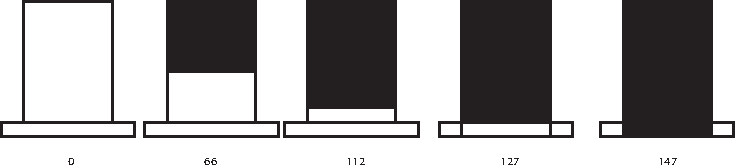
\includegraphics[width=\linewidth]{./resources/Asset 5.pdf}
\caption{Second attempt; upper limit defined}\label{fig:Asset5}
\end{figure}

\begin{figure}
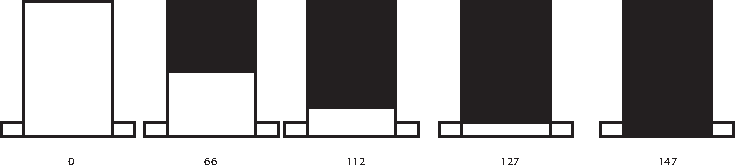
\includegraphics[width=\linewidth]{./resources/Asset 6.pdf}
\caption{`Imaginary ghost finger' single perspective}\label{fig:Asset6}
\end{figure}

\begin{figure}
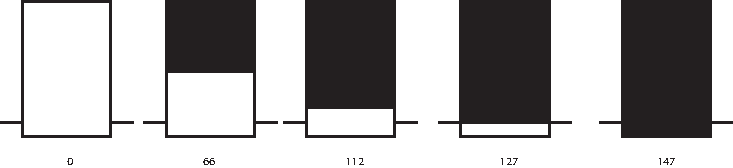
\includegraphics[width=\linewidth]{./resources/Asset 7.pdf}
\caption{Side view, upper limit defined}\label{fig:Asset7}
\end{figure}

\begin{figure}
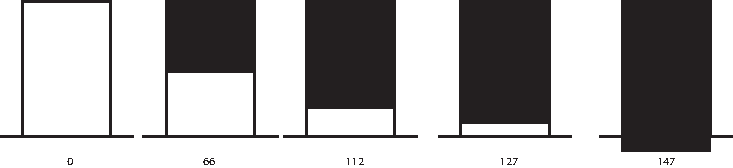
\includegraphics[width=\linewidth]{./resources/Asset 9.pdf}
\caption{Side view, without upper limit}\label{fig:Asset9}
\end{figure}


\section{Frank Zappa, Kate Soper, and Pepe Silvia}
David Dockery is a drummer that went viral years ago with his unique style of drumming in time to speech patterns of TV shows.\autocite[]{daviddockeryPepeSilviaDrums2017}
The effect is not dissimilar to that of Frank Zappa's song ``The Dangerous Kitchen'' amongst others, from his album ``The Man from Utopia''.\fxnote[]{zappa}
This effect of speech being done in time with the music can also be seen in Kate Soper's work ``Only the Words Themselves Mean What They Say''.\fxnote[]{soper}
Transcribing speech patterns and quantizing it to conform to a metrical grid is well established as a technique of introducing off-kilter rhythms that feel natural, 
however as Dockery's drumming shows, the works that are most in line with regular emotive speech contain multiple tempo and meter changes- 
showing that speech patterns are not typical iambic pentameter.

These transcriptions give us an insight into the mind of the composers, and I posit that the notated rhythms are notated thus not because the rhythms are important, but because the Western notation system does not give us adequate tools to notate speech-like cadences. 
In order to communicate the intended speech-like effect, the composers notate using the tools available, fitting their isochronous rhythms to the grid of Western notation.
This relies on either an explicit statement that the rhythms are unimportant, or the performer interpreting the subtext of the work correctly and surmising that without explicit direction.
This transcription process is lengthy, though, and when the intent is to mimic a relaxed and conversational style of speech, and not to reproduce those exact rhythms as notated, there is a degree of specificity of rhythm that is unnecessary, needlessly complicating the work.

My suggested notation is similar to non-barred music, as found in the works of Berio's Sequenzas.\fxnote[]{berio}
It involves the removal of barlines, and stems of notes. 
Rhythms are derived from the lyric line underneath the stave, as depicted in the below example.
This is not dissimilar to the approach used in Soper's work, wherein she notates the lyrics without any notes in the stave, and provides a time estimate above, as found in Lutoslawski's works.\fxnote{lutoslawski}
This is adequate when the work is not intended to have specific pitches (and thus fits the sprechstimme of `Only The Words Themselves Mean What They Say' quite well), but falls flat where pitch material is needed.


One of the issues with this is that it assumes both a level of flexibility in the rhythms, and a level of uniformity in how performers will interpret it; if the performer differs dramatically from the composer's rough intended idea, the work may fall out of `sync' with itself.
Mitigating this is the second version of notation, in which the beams are slightly wavy, contouring in the same manner as the \(\approx{}\) symbol. 
This reference to a pre-existing symbol for the notation of `approximately' is intended to aid comprehension by not reinventing the wheel.
This wavy-beamed notation can be used in existing Western style barred music, as well as convey a rough sense of intended rhythm when it differs from how a text would be spoken out loud.
This is useful because it gives the composer a way to `override' the performer's natural diction, without retreating back to the traditional Western notation system, which as discussed, is sometimes not suited for the notation of unfixed rhythms.

Composers that wish for a slightly more granular level of control of the rhythms can use the modified staving as notated \hl{FINISH SENTENCE}

One of the benefits of this notation system is that it maintains compatibility with the traditional Western notation system, and can be \hl{FINISH SENTENCE}

The simplest and most evident example of this technique's potential is when it is used with an instrument that can be spoken into, such as the recorder and most wind instruments. 
In the example work provided, the text is legible, but also can be used in tandem with regular notation systems, in a manner similar to that of Lutoslawski's stochastic aleatoricism.\fxnote{lutoslawski}
Like Lutoslawski's system, there is \hl{FINISH SENTENCE}

\subsection{Speech, Rhythm, and Music}
There is a long history of where speech and music intersect, at the crossroads of rhythm. 
Many languages are tonal, and thus pitch can also play a part in the meaning of the speech. 
However, we will just be looking at how speech interacts with music within the perimeter of English, for the purposes of this article. 

Speech is naturally coded into stressed and unstressed pairs, which help define the flow. 
Using Jassem's system of rhythmic organisation, the Narrow Rhythm Unit (NRU) is described as one stressed syllable and any number of following unstressed syllables belonging to the same word.\autocite[]{hillResultsPreliminaryStudy1977}
All the other unstressed syllables which are not part of the NRU belong to the anacrusis (ANA). 

Using this system, we have a convenient way for a composer to anticipate roughly the duration of their various words; anacruses are pronounced as quickly as possible, while the NRU is isochronous, with the speaker attempting to align them with an internal grid. 
Languages that make use of syllable based timing would necessitate a different notation system, but for English texts, it makes sense to exploit its inherent stress timing. 
These stress timings can be used as a method of applying another degree of control over the interpretation of the text, where the composer is able to anticipate lexical stress with a relatively high degree of confidence, whereas the prosodic stress variabilities can be mitigated with formatting techniques that are found in regular text script.
Bold fonts, italicization, parentheses, and a host of other notational elements can be used to ensure the stress is placed in the right place. 
This notations serve both as a means of enforcing correct interpretation (``I didn't say she stole my coat'' can have any word stressed for a different meaning), and as a means of enforcing correct rhythmic placement.

Notation often seeks to emulate the cadences of speech, and there has been much research into how speech falls into a natural iambic pentameter of sorts. 
Music notation is gridded, with on-beats and off-beats, and notating rhythms which fall off the tongue easily can turn into a very complex affair, with a lot of black ink devoted to ensuring that the rhythms do not lock into the grid in predictable fashions. 
Lutoslawski uses stochastic aleatory in a somewhat similar fashion, using repetitions which do not necessarily ``lock in'' to the grid.

One of the useful aspects of this is that it augments the rhythmic channel with additional subtextual information-- a performer that is taking the rhythmic information from a text concerned with anger would conceivably perform a more emotional rendition than one in which the rhythmic information was communicated with standard staff notation.

The isochrony hypothesis states that humans innately impose a rhythmic grid onto sound in order to parse and process it, dividing it into common integers such as 2, 3, 4, 8. 
In the absence of a consensus as to the relation of isochronous beat and stress boundaries, the human internal voice can achieve a similar effect, with a greater degree of variability from person to person-- 
where there is no clear beat structure, speech is typically in iambic pentameter, and can act as a surrogate, with a high degree of stochastic variation based both on the person and their diction. 

This is distinct from Sprechstimme and recitative because the pitch content is defined, but the rhythmic content is not, and is derived from the player; 
there's some semblance of predictability with how a performer will likely perform it since there are only so many ways to say ``How kind of you to let me come'', but the precise timings will likely be different with every performer, and likely differ every time a performer plays the work. 

Recitative is similar, but pre-biases the performer towards a gridded treatment of the musical material which I posit would be less of an issue if the work had untimed notation. 

The use of the barred staff notation system predisposes a performer (typically singer) to work within the bars- granted, the performer may use rubato and fall out of sequence with the rest of the ensemble, but the end result is almost always the performer falling back in time with the ensemble. 
This is fine, but does not quite meet the goals.

Proportional notation as seen in Berio's Sequenza for Flute has its own shortcomings; the stemmed notation poses no significant benefit, and does not diverge quite cleanly from traditional notation. 
On first glance, the work can appear to simply be poorly engraved, an issue which the speech-notation system avoids.

Perhaps the most closely aligned is the system of Gregorian Chant, in which notation is achieved through neumes. 
However, the neumal system is typically reliant on a conductor guiding the performers in unison; the gridded system still exists, it is just superimposed on the music by the players.

The most useful circumstances for this form of non-timed notation, or ``Words Without Songs'' is likely in the application of poetry or monologues. 
Words with rhyming conventions are naturally predisposed to adopting a gridding, which may render the use of this non-timed notation pointless. 
Speeches, poems, and other forms of text which do not make use of iambic pentameter will therefore manifest a more distinctly different rhythmic fingerprint than rhymed lyrics. 

Using non-timed notation, we can explore exciting possibilities by imbuing our performers with a degree of independence in group contexts; 
they have the freedom to play rhythms at their own pace. 
Additionally, the addition of another information channel means that they will be able to derive further meaning from the work. 
Consider the impact of a quartet that is playing a traditional call and response type of dialogue, when they are given ``lyrics'' for their music, which will directly inform their mindset and performance. 
With the addition of words without songs, an argument between two voices is literalised, and could only benefit from the change, bringing with it an added dimension for performers to explore. \hl{FINISH ARGUMENT}

\section{how to decay gracefully}

Using this non-timed notation system, I created my first exploratory score, titled `how to decay gracefully', a piece for solo recorder with text from the eponymous artwork by Samantha Hensley.\fxnote{TODO add Hensley}
This was a `dipping the toes into the water' sort of approach, as I also wanted to explore several other techniques (namely, speaking through the instrument, as well as the finger-in notation that was previously explored). 
Applying the text, which is a poem that appears at the top of the artwork, was a simple affair. 
For textural interest, I interspersed the monologue with several non-text-derived phrases, demonstrating the inter-compatibility of the system of non-timed notation.
The piece ends with the repeated phrase `lie still.' which I instructed the performer to say aloud. 
I found this to be an extremely effective instigator of unconscious minute differences in playing; 
while performing the piece, I did not notice that I would add emphasis or change the timbre of the spoken word, and the performer that recorded it for me, Claire Farrell, did this too.

\section{Interfaces}
We find that a schema or interface is necessary in order to parse the various notational aspects of sheet music, so that there is no data loss upon mutation of the interface.
What this means is that we need to understand what every part of a piece of sheet music (and the notation on it) communicates to the interpreter in order to be able know what can be changed.
Without an understanding of the interface, a composer may remove an element that may seem unimportant (beams on notes, for example), and then find that the interface no longer communicates an element that is important to their composition (without beams, rhythmic information is lost).
Thus, in order to make new methods of interacting with the score interface possible, we must first understand what the score interface is, and how we parse it.
Composers seeking to make use of emerging technologies, such as Alternate Reality, Virtual Reality, 3D effects, animated scores, interactive scores, or other as of yet unimagined ways of presenting instructions will derive the most benefit from this.
However, composers that stay closer to the classical art music tradition will still find use for the delineation of the function of each element of a score.

Defining terms for the interface is difficult, and there is cultural and semantic baggage no doubt associated with each and every term.
Creating a new word that is free of any context would be a double edged sword, where the reader lacks the real-world applicability of a stand-in term to define the meta-object.
Phrases such as `score' have connotations which would assist in the parsing of contextual meaning. 
However, assigning the same word to the interface as the physical object that it references is sure to be confusing.
Therefore, we need to use a term that is not already in use in a musical context, but has the assistive connotations that a similar term may have. 
It is for this reason that `interface' is a prime candidate for the way in which we communicate our musical ideas to the interpreter. 
The specific `musical score' can have its definition taken from the artistic world; `canvas' is a suitable choice, as it evokes a sense of a physical, tangible item to be painted upon.
The content of the canvas can be 

Mock example: 

% ScoreInterface {
%     methods: {
%         visual: {
%             mode: VisualMode
%             
%             isAnimated: boolean
%             isInteractive: boolean
%             isDynamic: boolean
%             is
%         }
%     }
%     interpreter: Performer
% }

% Audience {

% }

% Performer {

% }
% \include{mainmatter/conclusion}

\backmatter{}

\begin{appendixes}
    % % app0.tex (file to switch to appendix mode)
% No need to alter this file...
\newpage
\newcommand{\HRule}[1]{\rule{\linewidth}{#1}}
\newcommand\invisiblechapter[1]{%
  \refstepcounter{chapter}%
  \addcontentsline{toc}{chapter}{\protect\numberline{\thechapter}#1}%
  \chaptermark{#1}}
\appendix\appendixpage\addappheadtotoc\space


    % % app5.tex
\chapter{Multiphonic Fingering Chart}\label{app:Multiphonic Fingering Chart}
This is a way that you can include a long pdf.
\includepdf[pages=-,pagecommand={}]{./resources/multiphonicFingeringChart.pdf}
    % % app1.tex (file to switch to appendix mode)
% \newpage

% % \invisiblechapter{\violinPiece}
% \chapter[\violinPiece]{}


% \vspace*{3cm}
% \begin{center}
% \textsc{for solo recorder}
% \vspace*{3.5cm}

% \HRule{0.5pt}


% \LARGE \textbf{\uppercase{\violinPiece}}
% \HRule{2pt}

% \vspace{1.3cm}

% \normalsize February, 2021
% \date{}

% \vspace*{5\baselineskip}

% Rhys Gray

% \end{center}
% \newpage
% \section*{Program Notes}
% % \violinPiece\space is a solo work for violin that explores \hyperref[sec:half-harmonics]{half-harmonics}.
% It is a non-programmatic work, and the title was inspired by a question that my supervisor posed to me while I sought ethics approval for my exegesis; a simple phrase laden with possible contexts, spurring the imagination to try and complete the meaning.

% % It is, in a way, an etude, treating the half-harmonics in a way similar to those found in Sciarrino's \hyperref[fig:sciarrinoExcerpt]{\emph{6 Caprricio for violin}}. 
% Half-harmonics are produced by applying left hand finger pressure halfway between that required to create a harmonic, and a \emph{normale} sound. 
% The sound that is produced should be a mixture of the stopped string pitch, the harmonic pitch, and a resistant, slightly noisy quality.
% % They are notated in the score as a half-filled diamond notehead.

% \section*{Notation}
% \begin{itemize}

%     \item Half-harmonics are notated in the score as a half-filled diamond notehead.
%     \item Arrows denote gradual transitions to the technique that the arrow is pointing to.\begin{itemize}
%         \item Arrows between notes denote transitions between the types of notes (i.e.\ \emph{normale} to harmonic finger pressure.)
%       \end{itemize}
%     % \item sp denotes \emph{sul ponticello}.
%     % \item msp denotes \emph{molto sul ponticello}.
%     % \item similarly, st denotes \emph{sul tasto}, and mst denotes \emph{molto sul tasto}
% \end{itemize}

\newpage\label{app:howtodecaygracefullyscore}
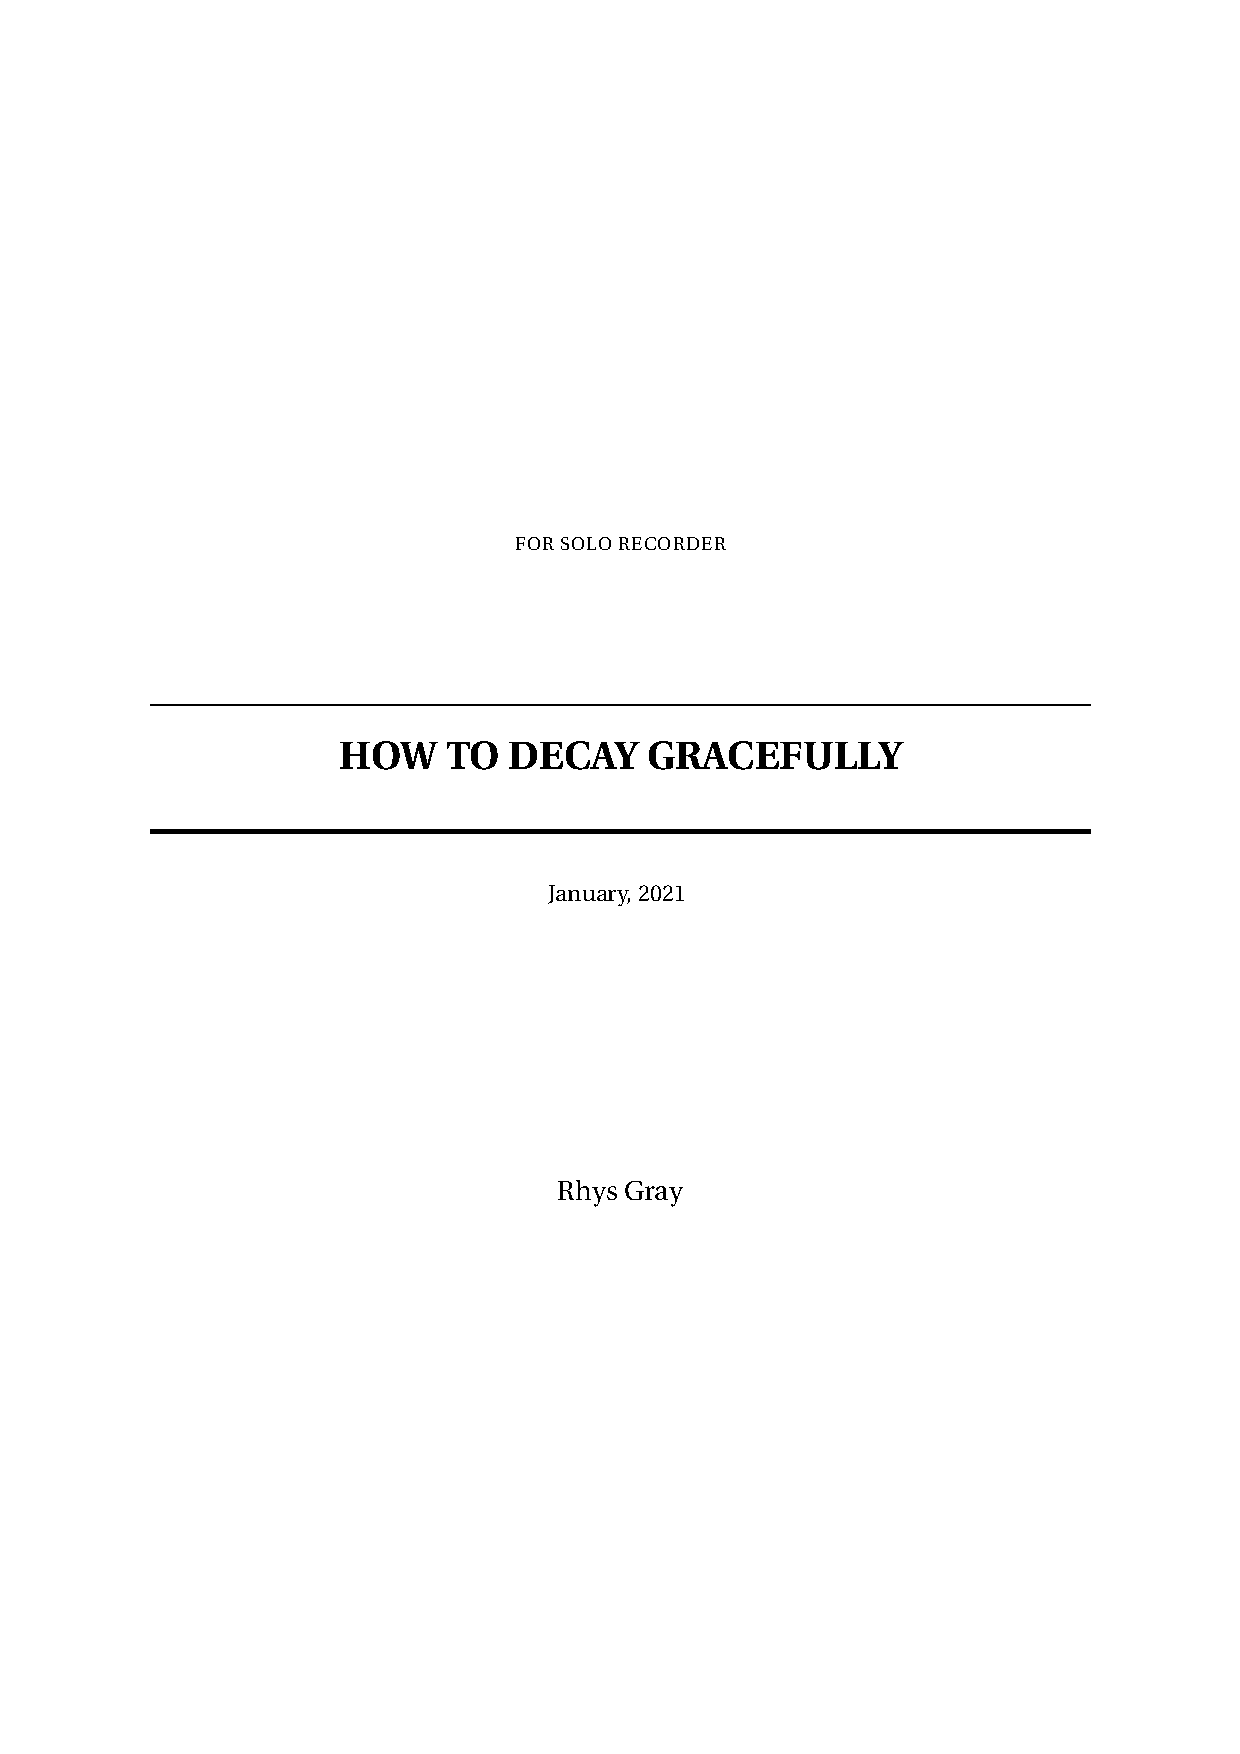
\includepdf[pages=-,pagecommand={}]{./resources/compositions/howtodecaygracefully.pdf}
    % % app2.tex (file to switch to appendix mode)

\chapter[\violaPiece]{}

\vspace*{3cm}
\begin{center}
\textsc{for solo viola}

\vspace*{3.5cm}

\HRule{0.5pt}


\LARGE \textbf{\uppercase{\violaPiece}}
\HRule{2pt}

\vspace{1.3cm}

\normalsize October, 2019
\date{}

\vspace*{5\baselineskip}

Rhys Gray

\end{center}
\newpage
\newpage

\section*{Program Notes}
\violaPiece\space is a piece for solo viola, written to explore the lower register of the viola using \hyperref[sec:subharmonics]{subharmonics} juxtaposed with upper harmonics. 

Subharmonics are achieved through precise control of torsional oscillation, which usually produces the sound of an amateur string player's heavy handed, slow bowing. 

To play subharmonics, one should place the bow at the 6th partial of the harmonic series of the fingered pitch, and bow with excessive pressure and an absolutely consistent speed. 
The increased pressure will distort the vibration of the string, producing a phase loop which, in turn, produces the subharmonic. 


The production of subharmonics can be aided by using older strings (which work better due to fats building up on the strings). 
Making a counter-clockwise half-twist in the string can also make it easier to produce octave and major second subharmonics (additional twists can help achieve lower subharmonics, at the expense of higher ones).

\section*{Notation}
\begin{itemize}

    \item Subharmonics are notated in the score using a square notehead for the fingering, with a small notehead at the desired resultant pitch. Where additional clarification is needed, `sh' is placed above.
    \item Arrows denote gradual transitions to the technique that the arrow is pointing to.\begin{itemize}
        \item Arrows between notes denote transitions between the types of notes (i.e.\ \emph{normale} to harmonic finger pressure.)
      \end{itemize}
    \item sp denotes \emph{sul ponticello}.
    \item msp denotes \emph{molto sul ponticello}.
    \item similarly, st denotes \emph{sul tasto}.
    \item n denotes \emph{normale}.
    \item Feathered beams denote a gradual acceleration to a tremolo.
\end{itemize}

\newpage\label{app:violaPiece Score}

% \includepdf[pages=-,pagecommand={},width=\textwidth]{./resources/compositions/violin.pdf}
\includepdf[pages=-,pagecommand={}]{./resources/compositions/viola.pdf}
    % % app2.tex (file to switch to appendix mode)

\chapter[\celloPiece]{}

\vspace*{3cm}
\begin{center}
\textsc{for solo violoncello}

\vspace*{3.5cm}

\HRule{0.5pt}


\LARGE \textbf{\uppercase{\celloPiece}}
\HRule{2pt}

\vspace{1.3cm}

\normalsize October, 2019
\date{}

\vspace*{5\baselineskip}

Rhys Gray

\end{center}
\newpage
\newpage

\section*{Program Notes}
\celloPiece\space is a piece for solo violoncello, written to explore \hyperref[sec:multiphonics]{multiphonics}. 

Multiphonics are achieved through clusters of close harmonic nodes, and by playing a harmonic close to the highest partial.
  Note that not all of these pitches will actually sound in practice.
  
  Multiphonics are notated as a harmonic position using a diamond notehead, with an `M' above the note to be fingered.
  Where the string used is ambiguous, it is notated below the sounding pitch as a small, bracketed notehead.
  Precise tuning is given in cents, and unless otherwise notated, is intended for the first note that the multiphonic is attached to.\footnote{100 cents is equal to a semitone. Therefore, +51c is roughly equal to half a semitone sharp. Cents have been used due to their precision compared to more granular accidentals such as the quartertone sharp.}
  The theoretical sounding pitches are given in a bracketed staff above the main stave.
  % Above the sounding pitches, the sounding partials are given (i.e. M IV [4th + 13th + 9th + 15th + 5th]).

  The bow should exert slightly more pressure than usual and should be drawn with a consistent speed which should be slower than for harmonics.
  The location of the bow can encourage or discourage upper or lower partials, and experimentation should be done during the practice of this work to achieve the pitches desired.

\section*{Notation}
\begin{itemize}
  \item Multiphonics are denoted with a diamond notehead, marked with an M (see \autoref{fig:multiphonicsBassExample} for an example). 
  \begin{itemize}
    \item Precise tuning in cents (i.e. +41c) is provided to help the performer pitch the fingering required for the multiphonic to be produced.
    \item The multiphonic resultant pitches are notated at pitch in the \emph{suono reale} stave, with the cents tuning of the resultant pitches to the left or right of the notes.
  \end{itemize}
    \item Arrows denote gradual transitions to the technique that the arrow is pointing to.\begin{itemize}
      \item Arrows between notes denote transitions between the types of notes (i.e.\ \emph{normale} to harmonic finger pressure.)
    \end{itemize}
    \item n denotes \emph{normale}.
    % \item sp denotes \emph{sul ponticello}.
    % \item msp denotes \emph{molto sul ponticello}.
    % \item similarly, st denotes \emph{sul tasto}, and mst denotes \emph{molto sul tasto}
\end{itemize}

\newpage\label{app:celloPiece Score}
\includepdf[pages=-,pagecommand={}]{./resources/compositions/violoncello.pdf}
    % % app2.tex (file to switch to appendix mode)

\chapter[\bassPiece]{}

\vspace*{3cm}
\begin{center}
\textsc{for solo contrabass}

\vspace*{3.5cm}

\HRule{0.5pt}


\LARGE \textbf{\uppercase{\bassPiece}}
\HRule{2pt}

\vspace{1.3cm}

\normalsize October, 2019
\date{}

\vspace*{5\baselineskip}

Rhys Gray

\end{center}
\newpage
\newpage

\section*{Program Notes}
Inspired by the eponymous short story by Ray Bradbury, \bassPiece\space is a composition for solo contrabass, and uses \hyperref[sec:subharmonics]{subharmonics} and \hyperref[sec:multiphonics]{multiphonics}. 
Similarly like the namesake, this world is filled with danger but also beauty. 
It is non-programmatic, and my intent with Veldt was to create a soundworld and space that the performer was able to `roam around' in, and features several sections of improvisation on pitch-sets.

\subsubsection*{Subharmonics}
Subharmonics are achieved through precise control of torsional oscillation, which usually produces the sound of an amateur string player's heavy handed, slow bowing. 

To play subharmonics, one should place the bow at the 6th partial of the harmonic series of the fingered pitch, and bow with excessive pressure and an absolutely consistent speed. 
The increased pressure will distort the vibration of the string, producing a phase loop which, in turn, produces the subharmonic. 
The production of subharmonics can be aided by using older strings (which work better due to fats building up on the strings). 
Making a counter-clockwise half-twist in the string can also make it easier to produce octave and major second subharmonics (additional twists can help achieve lower subharmonics, at the expense of higher ones).

\subsubsection*{Multiphonics}
Multiphonics are achieved through clusters of close harmonic nodes, and by playing a harmonic close to the highest partial.
  Note that not all of these pitches will actually sound in practice.
  
  Multiphonics are notated as a harmonic position using a diamond notehead, with an `M' above the note to be fingered.
  Where the string used is ambiguous, it is notated below the sounding pitch as a small, bracketed notehead.
  Precise tuning is given in cents, and unless otherwise notated, is intended for the first note that the multiphonic is attached to.\footnote{100 cents is equal to a semitone. Therefore, +51c is roughly equal to half a semitone sharp. Cents have been used due to their precision compared to more granular accidentals such as the quartertone sharp.}
  The theoretical sounding pitches are given in a bracketed staff above the main stave.
  % Above the sounding pitches, the sounding partials are given (i.e. M IV [4th + 13th + 9th + 15th + 5th]).

  The bow should exert slightly more pressure than usual and should be drawn with a consistent speed which should be slower than for harmonics.
  The location of the bow can encourage or discourage upper or lower partials, and experimentation should be done during the practice of this work to achieve the pitches desired.

\section*{Notation}
\begin{itemize}

    \item Subharmonics are notated in the score using a square notehead for the fingering, with a small notehead at the desired resultant pitch. Where additional clarification is needed, `sh' is placed above.
    \begin{itemize}
      \item They are notated at pitch in the cue sized stave above, with a harmonic circle above them.
    \end{itemize}
    \item Multiphonics are denoted with a diamond notehead, marked with an M (see \autoref{fig:multiphonicsBassExample} for an example). 
    \begin{itemize}
      \item Precise tuning in cents (i.e. +41c) is provided to help the performer pitch the fingering required for the multiphonic to be produced.
      \item The multiphonic resultant pitches are notated at pitch in the cue sized stave above, with the cents tuning of the resultant pitches to the left or right of the notes.
    \end{itemize}
    \item Arrows denote gradual transitions to the technique that the arrow is pointing to.\begin{itemize}
      \item Arrows between notes denote transitions between the types of notes (i.e.\ \emph{normale} to harmonic finger pressure.)
    \end{itemize}
    \item Sounding pitch is provided in the ossia stave above.
    \item Bridge position is provided in the stave above, and denotes the vertical location of the bow. The bottom line is \emph{molto sul tasto} and the top line is \emph{molto sul ponticello}.
    \item For un-metered bars, approximate times are given above in seconds, and is linearly proportional (i.e.\ note spacing denotes approximate time.)
    \item Repeats are to be repeated for as long as instructed.
    % \item \emph{battuto} is letting the bow hit the string, with no horizontal movement.
    % \item \emph{gettato} is like battuto, but with a slight amount of horizontal movement.
    % \item \emph{jeté} is bouncing the bow on the string, letting gravity do the work in conjunction with horizontal movement.
    \item op denotes overpressure.
    \item sp denotes \emph{sul ponticello}.
    \item n denotes \emph{normale}.
    % \item msp denotes \emph{molto sul ponticello}.
    % \item similarly, st denotes \emph{sul tasto}, and mst denotes \emph{molto sul tasto}
\end{itemize}

\newpage\label{app:bassPiece Score}

% \includepdf[pages=-,pagecommand={},width=\textwidth]{./resources/compositions/violin.pdf}

\includepdf[pages=-,pagecommand={}]{./resources/compositions/bass.pdf}
    % \include{backmatter/appendixb}
\end{appendixes}

\printbibliography{}

\end{document}